\chapter{Løsningsimplementering}
Arbeidet i denne fasen går ut på å utrede en tiltaksplan og lage et forslag til hvordan dette skal implementeres. I den foregående fasen ble løsningene til rotårsakene identifisert. Kort oppsummert var disse en bevisstgjøringskampanje, krav om strengere passordkontroll, 2-faktor autentisering, enhetskontroll, utbedring av IT-reglement og anbefaling om passordmanager. 

\section{Trediagram}
For å få en oversikt over hva som må gjøres for å implementere tiltaksplanen bruker vi Trediagram til å dele opp aktivitetene og bestemme rekkefølgen. 

\subsection{Ønsket utbytte}
Ønsket utbytte ved å bruke trediagram er å redegjøre for og strukturere de aktiviteter som må gjøres for å innføre de spesifikke tiltakene. 

\subsection{Gjennomføring}
Gjennomføringen av trediagrammet startet med å gruppere hovedtiltak til rotårsaken, deretter ble hver aktivitet som må gjennomføres for at tiltaket skal bli gjennomført gruppert. Disse underpunktene ble gruppert etter hvilken rekkefølge de skal bli implementert slik at tiltaket er mulig å gjennomføre. 

\subsection{Resultater}
Dette ga oss en fullstendig plan over hvilke aktiviteter som må gjennomføres for at tiltaket skal bli implementert.

\begin{figure}[p] 
    \centering    
    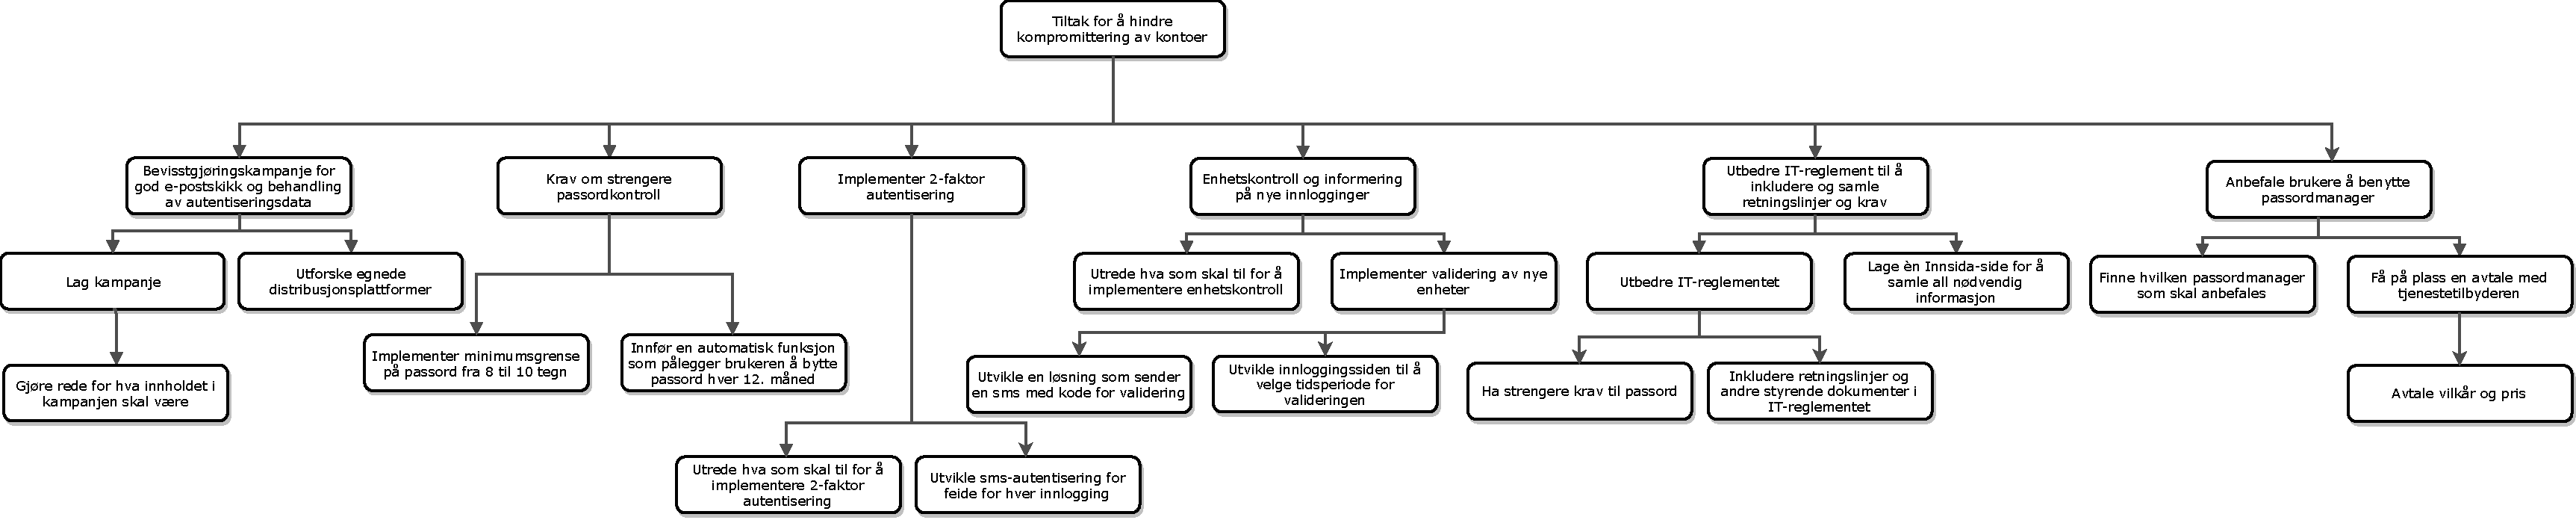
\includegraphics[scale=0.4, angle=90]{case_2/bilder/trediagram.pdf}
    \caption[Trediagram av tiltak case 2]{Trediagram av tiltak case 2}
    \label{fig:trediagram-case2}
\end{figure}


\subsection{Konklusjon av verktøy}
Dette verktøyet fungerte bra for å lage en plan til hvordan tiltakene skal bli implementert og hva som skal til for at tiltaket blir implementert. Trediagram er god måte å stykke opp arbeidsoppgavene for å skape en visuell prosess med oppgavene som må bli gjort for å nå målet. Det eneste som var problemet var at gruppen vår ikke har tilstrekkelig kunnskap om hvordan noen av tiltakene skal bli implementert.